%beamer

% TODO: Jede menge:
% Reguläre Ausdrüke in \rx umwandeln
% * Problem mit \rx fixen
% Folien ab "Zusammenhang..." besser einarbeiten
% Besser auf Zusammenhänge eingehen
% Besserer Aufbau der Beispiele und Aufgaben
% Strukturelle Induktion: Bessere Einführung, neues Beispiel, neue Aufgabe

% Define a global usable date. Must come before StyleTut
%\newcommand{\mydate}{03.02.2017}

% Comment/uncomment this line to toggle handout mode
%\newcommand{\handout}{}

% % \bigtimes abgeschrieben von http://tex.stackexchange.com/questions/14386/importing-a-single-symbol-from-a-different-font
% \DeclareFontFamily{U}{mathx}{\hyphenchar\font45}
% \DeclareFontShape{U}{mathx}{m}{n}{
%       <5> <6> <7> <8> <9> <10> gen * mathx
%       <10.95> mathx10 <12> <14.4> <17.28> <20.74> <24.88> mathx12
%       }{}
% \DeclareSymbolFont{mathx}{U}{mathx}{m}{n}
% \DeclareMathSymbol{\bigtimes}{\mathop}{mathx}{161}

\RequirePackage{xcolor}

\def\9{\square}
%\def\9{\blank}

% f"ur Aussagenlogik
\colorlet{alcolor}{blue}
\RequirePackage{tikz}
\usetikzlibrary{arrows.meta}
\newcommand{\alimpl}{\mathrel{\tikz[x={(0.1ex,0ex)},y={(0ex,0.1ex)},>={Classical TikZ Rightarrow[]}]{\draw[alcolor,->,line width=0.7pt,line cap=round] (0,0) -- (15,0);\path (0,-6);}}}
\newcommand{\aleqv}{\mathrel{\tikz[x={(0.1ex,0ex)},y={(0ex,0.1ex)},>={Classical TikZ Rightarrow[]}]{\draw[alcolor,<->,line width=0.7pt,line cap=round] (0,0) -- (18,0);\path (0,-6);}}}
\newcommand{\aland}{\mathbin{\raisebox{-0.6pt}{\rotatebox{90}{\texttt{\color{alcolor}\char62}}}}}
\newcommand{\alor}{\mathbin{\raisebox{-0.8pt}{\rotatebox{90}{\texttt{\color{alcolor}\char60}}}}}
%\newcommand{\ali}[1]{_{\mathtt{\color{alcolor}#1}}}
\newcommand{\alv}[1]{\mathtt{\color{alcolor}#1}}
\newcommand{\alnot}{\mathop{\tikz[x={(0.1ex,0ex)},y={(0ex,0.1ex)}]{\draw[alcolor,line width=0.7pt,line cap=round,line join=round] (0,0) -- (10,0) -- (10,-4);\path (0,-8) ;}}}
\newcommand{\alP}{\alv{P}} %ali{#1}}
%\newcommand{\alka}{\negthinspace\hbox{\texttt{\color{alcolor}(}}}
\newcommand{\alka}{\negthinspace\text{\texttt{\color{alcolor}(}}}
%\newcommand{\alkz}{\texttt{\color{alcolor})}}\negthinspace}
\newcommand{\alkz}{\text{\texttt{\color{alcolor})}}\negthinspace}
\newcommand{\AAL}{A_{AL}}
\newcommand{\LAL}{\hbox{\textit{For}}_{AL}}
\newcommand{\AxAL}{\hbox{\textit{Ax}}_{AL}}
\newcommand{\AxEq}{\hbox{\textit{Ax}}_{Eq}}
\newcommand{\AxPL}{\hbox{\textit{Ax}}_{PL}}
\newcommand{\AALV}{\hbox{\textit{Var}}_{AL}}
\newcommand{\MP}{\hbox{\textit{MP}}}
\newcommand{\GEN}{\hbox{\textit{GEN}}}
\newcommand{\W}{\ensuremath{\hbox{\textbf{w}}}\xspace}
\newcommand{\F}{\ensuremath{\hbox{\textbf{f}}}\xspace}
\newcommand{\WF}{\ensuremath{\{\W,\F\}}\xspace}
\newcommand{\val}{\hbox{\textit{val}}}
\newcommand{\valDIb}{\val_{D,I,\beta}}

\newcommand*{\from}{\colon}

% die nachfolgenden Sachen angepasst an cmtt
\newlength{\ttquantwd}
\setlength{\ttquantwd}{1ex}
\newlength{\ttquantht}
\setlength{\ttquantht}{6.75pt}
\def\plall{%
  \tikz[line width=0.67pt,line cap=round,line join=round,baseline=(B),alcolor] {
    \draw (-0.5\ttquantwd,\ttquantht) -- node[coordinate,pos=0.4] (lll){} (-0.25pt,-0.0pt) -- (0.25pt,-0.0pt) -- node[coordinate,pos=0.6] (rrr){} (0.5\ttquantwd,\ttquantht);
    \draw (lll) -- (rrr);
    \coordinate (B) at (0,-0.35pt);
  }%
}
\def\plexist{%
  \tikz[line width=0.67pt,line cap=round,line join=round,baseline=(B),alcolor] {
    \draw (-0.9\ttquantwd,\ttquantht) -- (0,\ttquantht) -- node[coordinate,pos=0.5] (mmm){} (0,0) --  (-0.9\ttquantwd,0);
    \draw (mmm) -- ++(-0.75\ttquantwd,0);
    \coordinate (B) at (0,-0.35pt);
  }\ensuremath{\,}%
}
\let\plexists=\plexist
\newcommand{\NT}[1]{\ensuremath{\langle\mathrm{#1} \rangle}}

\newcommand{\CPL}{\text{\itshape Const}_{PL}}
\newcommand{\FPL}{\text{\itshape Fun}_{PL}}
\newcommand{\RPL}{\text{\itshape Rel}_{PL}}
\newcommand{\VPL}{\text{\itshape Var}_{PL}}
\newcommand{\ATer}{A_{\text{\itshape Ter}}}
\newcommand{\ARel}{A_{\text{\itshape Rel}}}
\newcommand{\AFor}{A_{\text{\itshape For}}}
\newcommand{\LTer}{L_{\text{\itshape Ter}}}
\newcommand{\LRel}{L_{\text{\itshape Rel}}}
\newcommand{\LFor}{L_{\text{\itshape For}}}
\newcommand{\NTer}{N_{\text{\itshape Ter}}}
\newcommand{\NRel}{N_{\text{\itshape Rel}}}
\newcommand{\NFor}{N_{\text{\itshape For}}}
\newcommand{\PTer}{P_{\text{\itshape Ter}}}
\newcommand{\PRel}{P_{\text{\itshape Rel}}}
\newcommand{\PFor}{P_{\text{\itshape For}}}

\newcommand{\plka}{\alka}
\newcommand{\plkz}{\alkz}
%\newcommand{\plka}{\plfoo{(}}
%\newcommand{\plkz}{\plfoo{)}}
\newcommand{\plcomma}{\hbox{\texttt{\color{alcolor},}}}
\newcommand{\pleq}{{\color{alcolor}\,\dot=\,}}

% MODIFIED (DJ)
% previously: \newcommand{\plfoo}[1]{\mathtt{\color{alcolor}#1}}
\newcommand{\plfoo}[1]{\texttt{\color{alcolor}#1}}

\newcommand{\plc}{\plfoo{c}}
\newcommand{\pld}{\plfoo{d}}
\newcommand{\plf}{\plfoo{f}}
\newcommand{\plg}{\plfoo{g}}
\newcommand{\plh}{\plfoo{h}}
\newcommand{\plx}{\plfoo{x}}
\newcommand{\ply}{\plfoo{y}}
\newcommand{\plz}{\plfoo{z}}
\newcommand{\plR}{\plfoo{R}}
\newcommand{\plS}{\plfoo{S}}

\newcommand{\bv}{\mathrm{bv}}
\newcommand{\fv}{\mathrm{fv}}

%\newcommand{\AxAL}{\hbox{\textit{Ax}}_{AL}}
%\newcommand{\AALV}{\hbox{\textit{Var}}_{AL}}

%\renewcommand{\#}[1]{\literal{#1}}
\newcommand{\A}{\mathcal{A}}
\newcommand{\Adr}{\text{Adr}}
\newcommand{\ar}{\mathrm{ar}}
\newcommand{\ascii}[1]{\literal{\char#1}}
%\newcommand{\assert}[1]{\text{/\!\!/\ } #1}
\newcommand{\assert}[1]{\colorbox{black!7!white}{\ensuremath{\{\;#1\;\}}}}
\newcommand{\Assert}[1]{$\langle$\textit{#1}$\rangle$}
\newcommand{\B}{\mathcal{B}}
\newcommand{\bfmod}{\mathbin{\kw{ mod }}}
\newcommand{\bb}{{\text{bb}}}
\def\bottom{\hbox{\small$\pmb{\bot}$}}
\newcommand{\card}[1]{|#1|}
%\newcommand{\cod}{\mathop{\text{cod}}}  % ist in thwmathabbrevs
\newcommand{\Conf}{\mathcal{C}}
\newcommand{\define}[1]{\emph{#1}}
%\renewcommand{\dh}{d.\,h.\@\xspace}
%\newcommand{\Dh}{D.\,h.\@\xspace}
%\newcommand{\engl}[1]{engl.\xspace\emph{#1}}
\newcommand{\eps}{\varepsilon}
%\newcommand{\evtl}{evtl.\@\xspace}
\newcommand{\fbin}{\text{bin}}
\newcommand{\finv}{\text{inv}}
\newcommand{\fnum}{\text{num}}
\newcommand{\fNum}{{\text{Num}}}
\newcommand{\frepr}{\text{repr}}
\newcommand{\fRepr}{\text{Repr}}
\newcommand{\fZkpl}{\text{Zkpl}}
\newcommand{\fLen}{\text{Len}}
\newcommand{\fsem}{\text{sem}}
\providecommand{\fspace}{\mathord{\text{space}}}
\providecommand{\fSpace}{\mathord{\text{Space}}}
\providecommand{\ftime}{\mathord{\text{time}}}
\providecommand{\fTime}{\mathord{\text{Time}}}
\newcommand{\fTrans}{\text{Trans}}
\newcommand{\fVal}{\text{Val}}

% MODIFIED (DJ)
\newcommand{\Val}{\text{Val}}

%\def\G{\mathbb{Z}}
\newcommand{\HT}[1]{\normalfont\textsc{HT-#1}}
\newcommand{\htr}[3]{\{#1\}\;#2\; \{#3\}}
\newcommand{\Id}{\text{I}}
%\newcommand{\ie}{i.\,e.\@\xspace}
\newcommand{\instr}[2]{\texttt{#1}\ \textit{#2}}
\newcommand{\Instr}[2]{\texttt{#1}\ \textrm{#2}}
\newcommand{\instrr}[3]{\texttt{#1}\ \textit{#2}\texttt{(#3)}}
\newcommand{\Instrr}[3]{\texttt{#1}\ \textrm{#2}\texttt{(#3)}}
\newcommand{\io}{\!\mid\!}
\usepackage{KITcolors}
\newcommand{\literal}[1]{\hbox{\textcolor{blue!95!white}{\textup{\texttt{\scalebox{1.11}{#1}}}}}}
%\newcommand{\literal}[1]{\hbox{\textcolor{KITblue!80!black}{\textup{\texttt{#1}}}}}
\def\kasten#1{\leavevmode\literal{\setlength{\fboxsep}{1pt}\fbox{\vrule  width 0pt height 1.5ex depth 0.5ex #1}}}
\newcommand{\kw}[1]{\ensuremath{\mathbf{#1}}}
\newcommand{\lang}[1]{\ensuremath{\langle#1\rangle}}
%\newcommand{\maw}{m.\,a.\,w.\@\xspace}
%\newcommand{\MaW}{M.\,a.\,w.\@\xspace}
\newcommand{\mdefine}[2][FOOBAR]{\define{#2}\def\foobar{FOOBAR}\def\optarg{#1}\ifx\foobar\optarg\def\optarg{#2}\fi\graffito{\optarg}}
\newcommand{\meins}{\rotatebox[origin=c]{180}{1}}
\newcommand{\Mem}{\text{Mem}}
\newcommand{\memread}{\text{memread}}
\newcommand{\memwrite}{\text{memwrite}}
\providecommand{\meta}[1]{\ensuremath{\langle}\textit{#1}\ensuremath{\rangle}}
%\newcommand{\N}{\mathbb{N}}
\newcommand{\NP}{\mathbf{NP}}
\newcommand{\Nadd}{N_{\text{add}}}
\newcommand{\Nmult}{N_{\text{mult}}}
% MODIFIED (DJ): added \!, mathcal{O}
\newcommand{\Oh}[1]{\mathcal{O}\!\left(#1\right)}
\newcommand{\Om}[1]{\Omega\!\left(#1\right)}
\newcommand{\personname}[1]{\textsc{#1}}
\newcommand{\regname}[1]{\texttt{#1}}
\newcommand{\mima}{\textsc{Mima}\xspace}
\newcommand{\mimax}{\textsc{Mima-X}\xspace}

\def\Pclass{\text{\bfseries P}}
\def\PSPACE{\text{\bfseries PSPACE}}

\newcommand{\SPush}{\text{push}}
\newcommand{\SPop}{\text{pop}}
\newcommand{\SPeek}{\text{peek}}
\newcommand{\STop}{\text{top}}
\newcommand{\STos}{\text{\itshape tos}}
\newcommand{\SBos}{\text{\itshape bos}}

%\newcommand{\R}{\mathbb{R}}
\newcommand{\Rnullplus}{\R_0^{+}}
\newcommand{\Rplus}{\R_{+}}
\newcommand{\resp}{resp.\@\xspace}
\newcommand{\Sem}{\text{Sem}}
\newcommand{\sgn}{\mathop{\text{sgn}}}
\newcommand{\sqbox}{\mathop{\raisebox{-6.2pt}{\hbox{\hbox to 0pt{$^{^{\sqcap}}$\hss}$^{^{\sqcup}}$}}}}
\newcommand{\sqleq}{\sqsubseteq}
\newcommand{\sqgeq}{\sqsupseteq}
% MODIFIED (DJ): added \!
\newcommand{\Th}[1]{\Theta\!\left(#1\right)}
%\newcommand{\usw}{usw.\@\xspace}
\newcommand{\V}[1]{\hbox{\textit{#1}}}
\newcommand{\x}{\times}
\newcommand{\ZK}{\mathbb{K}}
%\newcommand{\Z}{\mathbb{Z}}
\newcommand{\zB}{z.\,B.\@\xspace}
\newcommand{\ZB}{Z.\,B.\@\xspace}
% \newcommand{\bb}{{\text{bb}}}
% \def\##1{\hbox{\textcolor{darkblue}{\texttt{#1}}}}
% \def\A{\mathcal{A}}
% \newcommand{\0}{\#0}
% \newcommand{\1}{\#1}
% \newcommand{\Obj}{\text{Obj}}
% \newcommand{\start}{\mathop{\text{start}}}
% \newcommand{\compactlist}{\addtolength{\itemsep}{-\parskip}}
% \newcommand{\fval}{\text{val}}
% \newcommand{\lang}[1]{\ensuremath{\langle#1\rangle}}
% \newcommand{\io}{\!\mid\!}
% \def\sqbox{\mathop{\raisebox{-6.2pt}{\hbox{\hbox to 0pt{$^{^{\sqcap}}$\hss}$^{^{\sqcup}}$}}}}
% \def\sqleq{\sqsubseteq}
% \def\sqgeq{\sqsupseteq}
\def\Td{T_{\overline{d}}}
% \newcommand{\csym}[1]{\ensuremath{\#{c}_{\#{\hbox{\scriptsize #1}}}}}
% \newcommand{\F}{\ensuremath{\mathcal{F}}}
% \newcommand{\fsym}[2]{\ensuremath{\#{f}^{\#{\hbox{\scriptsize #1}}}_{\#{\hbox{\scriptsize #2}}}}}
% \newcommand{\rsym}[2]{\ensuremath{\#{R}^{\#{\hbox{\scriptsize #1}}}_{\#{\hbox{\scriptsize #2}}}}}
% \newcommand{\xsym}[1]{\ensuremath{\#{x}_{\#{\hbox{\scriptsize #1}}}}}
% \newcommand{\I}{\mathcal{I}}
% ********************************************************************

\usepackage{../TutTexbib/thwregex}

\newcommand{\nM}{\mathbb{M}}
\newcommand{\nR}{\mathbb{R}}
\newcommand{\nN}{\mathbb{N}}
\newcommand{\nZ}{\mathbb{Z}}
\newcommand{\nQ}{\mathbb{Q}}
\newcommand{\nB}{\mathbb{B}}
\newcommand{\nC}{\mathbb{C}}
\newcommand{\nK}{\mathbb{K}}
\newcommand{\nF}{\mathbb{F}}
\newcommand{\nG}{\mathbb{G}}
\newcommand{\nullel}{\mathcal{O}}
\newcommand{\einsel}{\mathds{1}}
\newcommand{\nP}{\mathbb{P}}
\newcommand{\Pot}{\mathcal{P}}
\renewcommand{\O}{\text{O}}

%\newcommand{\literal}[1]{\textcolor{blue}{\texttt{#1}}}
\newcommand{\realTilde}{\textasciitilde \ }
\newcommand{\setsize}[1]{\; \mid #1 \mid \; }

\definecolor{myRed}{RGB}{255,75,20}
\colorlet{myGreen}{KITpalegreen}

\newcounter{tfqtempcount}
\newcommand{\truefalseQ}[4]{
	\setcounter{tfqtempcount}{#1}
	\addtocounter{tfqtempcount}{1}
	\truefalseQuestion{#1}{\value{tfqtempcount}}{#2}{#3}{#4}
}
\newcommand{\truefalseQuestion}[5]{\item<#1-|handout:#1-> \color<#2-|handout:#2->{#3} #4 \qquad \visible<#2-|handout:#2->{#5}}

\newcommand{\boder}{\ensuremath{\textcolor{blue}{\vee}}\text{} }
\newcommand{\bund}{\ensuremath{\textcolor{blue}{\wedge}}\text{}}
\newcommand{\bimp}{\ensuremath{\textcolor{blue}{\to}}\text{}}
\newcommand{\bnot}{\ensuremath{\textcolor{blue}{\neg}}\text{}}
\newcommand{\bone}{\ensuremath{\textcolor{blue}{1}}\text{}}
\newcommand{\bzero}{\ensuremath{\textcolor{blue}{0}}\text{}}
\newcommand{\bleftBr}{\ensuremath{\textcolor{blue}{(}}\text{}}
\newcommand{\brightBr}{\ensuremath{\textcolor{blue}{)}}\text{}}

\newcommand{\summe}[2]{\sum\limits_{#1}^{#2}}
\newcommand{\limes}[1]{\lim\limits_{#1}}

\newcommand{\numpp}{\advance \value{weeknum} by -2 \theweeknum \advance \value{weeknum} by 2}
\newcommand{\nump}{\advance \value{weeknum} by -1 \theweeknum \advance \value{weeknum} by 1}

\newcommand{\mycomment}[1]{}

\newcounter{abc}
\newenvironment{alist}{
  \begin{list}{(\alph{abc})}{
      \usecounter{abc}\setlength{\leftmargin}{8mm}\setlength{\labelsep}{2mm}
    }
}{\end{list}}

\renewcommand{\mod}{\text{ \bf{mod} }}
\renewcommand{\div}{\text{ \bf{div} }}

%\newcommand{\sgn}{\text{sgn}}

% Toggle Handout mode by including this line before including style_tut:
% \newcommand{\handout}{}

%% Beamer-Klasse im korrekten Modus
\ifdefined \handout
\documentclass[handout]{beamer} % Handout mode
\else
\documentclass{beamer}
\fi


% Das ist der KIT-Stil
%\usepackage{../TutTexbib/beamerthemekit}
\usepackage[deutsch,titlepage0]{../TutTexbib/KIT/beamerthemeKITmod}
\TitleImage[width=\titleimagewd]{../figures/titlepage.jpg}
%\usetheme[deutsch,titlepage0]{KIT}

% Include PDFs
\usepackage{pdfpages}

% Libertine font (Original GBI font)
\usepackage{libertine}
%\renewcommand*\familydefault{\sfdefault}  %% Only if the base font of the document is to be sans serif

% Nicer math symbols
\usepackage{eulervm}
%\usepackage{mathpazo}

%% Deutsche Silbentrennung und Beschriftungen
\usepackage[ngerman]{babel}

%% UTF-8-Encoding
\usepackage[utf8]{inputenc}

\usepackage{csquotes}

%% Bibliotheken für viele mathematische Symbole
\usepackage{amsmath, amsfonts, amssymb}

%% Anzeigetiefe für Inhaltsverzeichnis: 1 Stufe
\setcounter{tocdepth}{1}

%% Schönere Schriften
\usepackage[TS1,T1]{fontenc}

%% Tabellen
\usepackage{array}
\usepackage{multicol}

%% Bibliothek für Graphiken
\usepackage{graphicx}

%% der wird sowieso in jeder Datei gesetzt
%%\graphicspath{{../figures/}}

%% Hyperlinks
\usepackage{hyperref}
% I don't know why, but this works and only includes sections and NOT subsections in the pdf-bookmarks.
\hypersetup{bookmarksdepth=subsection} 

%\usepackage{lmodern}
\usepackage{colortbl}
\usepackage[absolute,overlay]{textpos}
\usepackage{listings}
\usepackage{forloop}
%\usepackage{algorithmic} % PseudoCode package 

\usepackage{tikz}
\usetikzlibrary{matrix}
\usetikzlibrary{arrows.meta}
\usetikzlibrary{automata}
\usetikzlibrary{tikzmark}

% Needed for gbi-macros
\usepackage{xspace}

%%%%%%%%%%%% INHALT %%%%%%%%%%%%%%%%

%% Wochennummer
\newcounter{weeknum}

%% Titelinformationen
\title[GBI Tutorium, Woche \theweeknum]{Grundbegriffe der Informatik \\ Tutorium 36}
\subtitle{Termin \theweeknum \ | \mydate \\ Thassilo Helmold}
\author[Thassilo Helmold]{Thassilo Helmold}
\institute{KIT -- Karlsruher Institut für Technologie}
\date{\mydate}

%% Titel einfügen
\newcommand{\titleframe}{\frame{\titlepage}}

%% Alles starten mit \starttut{X}
\newcommand{\starttut}[1]{\setcounter{weeknum}{#1}\titleframe\frame{\frametitle{Inhalt}\tableofcontents} \AtBeginSection[]{%
\begin{frame}
	\tableofcontents[currentsection]
\end{frame}\addtocounter{framenumber}{-1}}}


\newcommand{\framePrevEpisode}{
	\begin{frame}
		\centering
		\textbf{In the previous episode of GBI...}
	\end{frame}
}

%% Legacy: Lastframe. Not for further usage!
\newcommand{\lastframe}[4]{\xkcdframe{#1}{#2}{#3}{#4}{}}
\newcommand{\xkcdframe}[5]{
	\frame[plain]{
		\vspace{-#2pt}
		\begin{figure}[H]
			\centering
			\includegraphics[scale=#1]{#3}
			\vspace{-7pt}
			\caption{ \texttt{\url{#4}} }
			\vspace{5pt}
			#5
		\end{figure} 
	}
}

%% Wörter
\newcommand{\code}[1]{$\mathbf{#1}$}

%% Sterne

\newcounter{starsc}
\newcommand{\stars}[1]{
	\hfill
	\begin{minipage}{100px}
		\forloop{starsc}{0}{\value{starsc} < #1}%
		{%
			\includegraphics[scale=0.05]{star-full.pdf} \hspace*{1px}
		}%
		\forloop{starsc}{\value{starsc}}{\value{starsc} < 5}%
		{%
			
\includegraphics[scale=0.05]{star-empty.pdf} \hspace*{1px}
		}
		\vspace*{2px}
	\end{minipage}
}

% No stars for me...
\renewcommand{\stars}[1]{}

\newcommand{\slideThanks}{
	\begin{frame}
		\frametitle{Danksagung}
		\begin{block}{}
			Dieser Foliensatz basiert in Teilen auf Folien von:\\[1em]
			Philipp Basler \\
			Nils Braun \\
			Dominik Doerner \\
			Ou Yue \\
		\end{block}
	\end{frame}
}

%% Verbatim
\usepackage{moreverb}
\graphicspath{{../figures/}}

\begin{document}
\starttut{13}

\framePrevEpisode

\begin{frame}{Rückblick: Laufzeitabschätzungen}
	\begin{itemize}[<+->]
		\item Asymptotisches Wachstum
		\item $O, \Theta, \Omega$
		\item Beweisverfahren
		\item Rechenregeln im O-Kalkül
	\end{itemize}
\end{frame}

\begin{frame}{Rückblick}
	\centering
	\includegraphics[scale=0.5]{laufzeit/polyVsExp}
\end{frame}

\begin{frame}{Wahr oder Falsch?}
	\TrueQuestionE{$x^4 \in \Oh{{(x^3)}^3}$}{ $\qquad {(x^3)}^3 = x^9$}
	\FalseQuestionE{$\sqrt{n} \in \Om{2^n}$}{}
	\TrueQuestionE{$log_{5000} n \in \Th{\log_2{n^4}}$}{ $\qquad \log_2{n^4} = 4 \cdot \log_2{n}$}
	\FalseQuestionE{$O(f_1) + f_2 = O(f_1 + f_2)$}{Aber: $O(f_1) + O(f_2) = O(f_1 + f_2)$}
\end{frame}

\begin{frame}{Wahr oder Falsch?}
	\FalseQuestion{Für zwei Funktionen $f, g$ gilt immer $f \preceq g$ oder $f \succeq g$}
	\medskip
	
	\visible<2>{
		Es gibt unvergleichbare Funktionen.
		\begin{align*}
		f &=
		\begin{cases}
		1 & \text{ falls $n$ gerade} \\
		n & \text{ falls $n$ ungerade} \\
		\end{cases} \\
		g &=
		\begin{cases}
		n & \text{ falls $n$ gerade} \\
		1 & \text{ falls $n$ ungerade} \\
		\end{cases} \\
		\end{align*}
		Es gilt \emph{nicht} $g\preceq f$, es gilt \emph{nicht} $f\preceq
		g$ und es gilt erst recht \emph{nicht} $f\asymp g$.
	}
\end{frame}


\begin{frame}{Logarithmen encore}
	Berechnet:
	\begin{align*}
	\log_5(25 \cdot 125) &= \visible<2->{\log_5(25) + \log_5(125) = 2+3 = 5}\\
	16^{\log_4(5)} &= \visible<3->{5^{\log_4(16)} = 5^2 = 25}
	\end{align*}
\end{frame}

\begin{frame}{Laufzeiten}
	\pause
	Lineare Suche: \pause $\Th{n}$ \\
	Binäre Suche:  \pause $\Th{\log n}$ \\
	Potenzmenge berechnen: \pause $\Th{2^n}$
\end{frame}

\section{Master-Theorem}

\begin{frame}{Teile und herrsche -- divide and conquer}
	\begin{itemize}
		\item Probleminstanz in kleinere Teile zerlegen
		\item Teile rekursiv nach gleichen Verfahren bearbeiten
		\item Aus Teilergebnissen Resultat rekonstruieren
	\end{itemize}
\end{frame}

\begin{frame}{Das Master-Theorem (einfache Form)}
	Situation aus dem Leben: 
	\begin{itemize}[<+->]
		\item Wir haben einen rekursiven Algorithmus $A(n)$ für die Problemgröße $n$
		\item Bei jedem Schritt wird das Problem um $b$ geteilt und es ergeben sich $a$ neue Probleminstanzen der Größe $n/b$
		\item Wie können die Laufzeit der jeweiligen \enquote{Auseinandernehmungs-} und \enquote{Zusammenführungsschritte} \textbf{linear} abschätzen.
	\end{itemize}
\end{frame}

\begin{frame}{Das Master-Theorem (einfache Form)}
	\includegraphics[scale=0.5]{laufzeit/masterTheorem}
\end{frame}

\begin{frame}{MT: Beispiele}
	Wir betrachten verschiedene Sortierverfahren:\\
	\bigskip
	
	\textbf{Mergesort}\\
	msort(L: Liste mit |L| = n):\\
		teile L in der Mitte auf in $L_1$ und $L_2$\\
		sortiere $L_1$ und $L_2$\\
		füge $L_1$ und $L_2$ in O($n$) zusammen\\
	\medskip
	
	$$r(n) = \pause \begin{cases}
	1 & n = 1\\
	c \cdot n + 2 \cdot r(n/2) & n > 1
	\end{cases}$$
	
	\pause
	Nach MT, Fall 2 also: $r(n) \in \Th{n \log n}$
\end{frame}

\begin{frame}{MT: Beispiele}
	Wir betrachten verschiedene Sortierverfahren:\\
	\bigskip
	
	\textbf{DoubleMergesort}\\
	dmsort(L: Liste mit |L| = n):\\
	teile L in der Mitte auf in $L_1$ und $L_2$\\
	sortiere $L_1$ und $L_2$ \textbf{jeweils zwei mal}\\
	\textit{Ja, das hat natürlich keinerlei Sinn und ist rein konstruiert}\\
	füge $L_1$ und $L_2$ in O($n$) zusammen\\
	\medskip
	
	$$r(n) = \pause \begin{cases}
	1 & n = 1\\
	c \cdot n + 4 \cdot r(n/2) & n > 1
	\end{cases}$$
	
	\pause
	Nach MT, Fall 3 also: $r(n) \in \Th{n^2}$
\end{frame}

\begin{frame}{MT: Beispiele}
	Wir betrachten verschiedene Sortierverfahren:\\
	\bigskip
	
	\textbf{Magicsort}\\
	msort(L: Liste mit |L| = n):\\
	teile L in der Mitte auf in $L_1$ und $L_2$\\
	sortiere $L_1$\\
	$L_2$ ist an dieser Stelle durch Magie bereits sortiert\\
	füge $L_1$ und $L_2$ in O($n$) zusammen\\
	\medskip
	
	$$r(n) = \pause \begin{cases}
	1 & n = 1\\
	c \cdot n + 1 \cdot r(n/2) & n > 1
	\end{cases}$$
	
	\pause
	Nach MT, Fall 1 also: $r(n) \in \Th{n}$
	\medskip
	
	\textbf{ACHTUNG:} Magicsort kann es nicht geben! In Algorithmen I:\\ 
	Untere Schranke für vergleichsbasiertes Sortieren ist $\Om{n \log n}$
\end{frame}


\begin{frame}{Limitierungen des MT}
	Das Master-Theorem ist mächtig, aber leider längst nicht so mächtig, wie der Name es vielleicht vermuten lässt.\\
	\pause
	Dieses (einfache) MT funktioniert nur bei sehr speziellen Rekkurenzformen (auch wenn diese häufig vorkommen).\\
	\pause
	Ein erweitertes MT wurde in der VL vorgestellt, ist aber auch nicht vollständig!\\
	\pause
	\medskip
	Bei ungleichen Aufteilungen hilft einem das MT überhaupt nicht weiter:\\
	Berechnet man $(n + 1)! = n! \cdot (n + 1)$, so kann die Laufzeit der Berechnung nicht mit dem MT abgeschätzt werden.
\end{frame}

\section{Automaten}

\begin{frame}{Endliche Automaten}
	Ein deterministischer endlicher Automat...
	\begin{itemize}
		\item besteht aus endlich vielen Zuständen
		\item ist zu jedem Zeitpunkt in \emph{genau einem} dieser Zustände
		\item wechselt bei Eingabe \emph{genau eines} Zeichens den Zustand in \emph{genau einen, definierten} Folgezustand
		\item und gibt dabei ein Wort als Ausgabe aus
	\end{itemize}

	Die gültigen \enquote{Zustandswechsel} sind als Zustandsübergänge definiert.
\end{frame}

\begin{frame}{Anwendungen}
	\begin{itemize}
		\item Getränkeautomaten
		\item Textsuche
		\item Textersetzung
	\end{itemize}

	Für Beispiele zur Textsuche und Textersetzung: Übung~12, WS~15/16
\end{frame}

\mycomment{ % As a source for copy/pasting:
\begin{tikzpicture}[->,>=stealth,shorten >=1pt,auto,node distance=2.8cm,
semithick,initial text={}]
\tikzstyle{every state}=[fill=red,draw=none,text=white]

\node[initial,state] (A)                    {$q_a$};
\node[state]         (B) [above right of=A] {$q_b$};
\node[state]         (D) [below right of=A] {$q_d$};
\node[state]         (C) [below right of=B] {$q_c$};
\node[state]         (E) [below of=D]       {$q_e$};

\path (A) edge              node {0,1,L} (B)
		  edge              node {1,1,R} (C)
(B) edge [loop above] node {1,1,L} (B)
	edge              node {0,1,L} (C)
(C) edge              node {0,1,L} (D)
	edge [bend left]  node {1,0,R} (E)
(D) edge [loop below] node {1,1,R} (D)
	edge              node {0,1,R} (A)
(E) edge [bend left]  node {1,0,R} (A);
\end{tikzpicture}	
}

\subsection{Mealy-Automaten}
\begin{frame}{Ein einfacher Automat}
	\begin{center}
		\begin{tikzpicture}[->,>=stealth,shorten >=1pt,auto,node distance=2.8cm,
			semithick,initial text={}]
			\tikzstyle{every state}=[]
			
			\node[initial,state] (A)                    {$a$};
			\node[state]         (M) [right of=A] 	    {$m$};
			
			\path (A) edge [loop above] node {\word 1|\word 0} (A)
			          edge [loop below]  node {\word 0|\word 1} (A)
			          edge 					  node {\word{2}|\word{X}} (M)
			      (M) edge [loop right] node {$\stackedtight{\word 0|\word X \\ \word 1|\word X \\ \word 2|\word X}$} (M);
			      %(M) edge [loop right] node {\word 1|\word X} (M)
			      %(M) edge [loop below] node {\word 2|\word X} (M);
		\end{tikzpicture}
	\end{center}
	\pause
	Eingabe: \word{011101} \?> Ausgabe: \word{100010} \\
	Eingabe: \word{011102} \?> Ausgabe: \word{10001X} \\
	Eingabe: \word{012101} \?> Ausgabe: \word{10XXXX} \\ \pause
	\smallskip
	\impl Der Automat negiert das Eingabewort bitweise. \\
	(Frisst er ne \word 2, so isser beleidigt. \smiley)
\end{frame}

\begin{frame}{Mealy-Automat}
	Bei einem Mealy-Automaten findet die Ausgabe \textbf{bei den Zustandsübergängen} statt.
	\begin{Definition}
		Ein \textbf{Mealy-Automat} $ A = (Z,z_0,X,f,Y,g)$ besteht aus...
		\begin{itemize}
			\item einer endlichen Zustandsmenge $Z$ 
			\item einem Startzustand $z_0$
			\item einem Eingabealphabet $X$ 
			\item einer Zustandsübergangsfunktion $f \from Z\times X \functionto Z $
			\item einem Ausgabealphabet $Y$
			\item einer Ausgabefunktion $g \from Z\times X \functionto Y^* $ 
		\end{itemize}						
	\end{Definition}
\end{frame}

\begin{frame}{}
	\begin{block}{Graphische Darstellung}
		\begin{itemize}
			\item Oft malt man Automaten hin. (Achtung: Die formale Schreibweise wird trotzdem auch im Studium verwendet! Also auswendig lernen!)
			\item Zustände sind \textbf{Knoten} und Übergänge sind \textbf{gerichtete Kanten} in einem Graphen. \\
			Kanten\textbf{beschriftung}: „$\langle\text{Eingabe}\rangle | \langle\text{Ausgabe}\rangle$“
			\item \textbf{Der Startzustand wird mit einem Pfeil \enquote{aus dem Nichts} gekennzeichnet!}  \pause
			\implitem \textbf{NICHT VERGESSEN!} Kostet sonst Punkte! \textbf{Immer!}
		\end{itemize}
		
	\end{block}
\end{frame}

\begin{frame}{Beispiel: Automatengraphen}
	%\vspace{-1\baselineskip} 
	%\hspace{-\baselineskip}
	\includegraphics[page=3,trim=18px 47px 18px 14px,clip]{U12.pdf}	
\end{frame}

%% Übung: Beispiel
%\setbeamercolor{background canvas}{bg=}


\begin{frame}{Eingabe eines Zeichens}
	Was ist die Zustandsübergangsfunktion $f$? \\ \pause
	\medskip
	Haben
	\begin{itemize}
		\item aktuellen Zustand $z \in Z$
		\item eingelesenes Zeichen $x \in X$
	\end{itemize}
	\impl $f$ liefert den Folgezustand $z_\text{neu}$, in welchem der Automat danach ist.\\
	\medskip
	Formell: $$ f(z,x) = z_\text{neu} $$ 
\end{frame}

\begin{frame}{Eingabe eines Wortes}
	Was machen wir mit ganzen Wörtern? \\ \pause
	Wir definieren uns ganz analog
	\begin{block}{Zustandsübergangsfunktion extended}
	\begin{align*}
		 	f_*(z,\eps) &:= z \\
		 	\forall w\in X^* , \, x\in X : \quad  f_*(z,wx) &:= f\left(f_*(z,w),x\right) 
	\end{align*}
	\end{block}
	\pause Was macht diese Funktion? \\ \pause
	\medskip
	Haben
	\begin{itemize}
		\item aktuellen Zustand $z \in Z$
		\item eingelesenes Wort $w \in X^*$
	\end{itemize}
	\impl $f_*$ liefert den \textbf{Endzustand} $z_\text{ende}$, in welchem der Automat \textbf{nach dem Wort} dann ist.
	Formell: $$ f_*(z,w) = z_\text{ende} $$
	%Bei Eingabe eines Wortes $w$ und Anfangszustand $z$ gibt sie den Zustand $z' = f_*(z,w)$ aus, in dem der Automat enden wird. 
\end{frame}
	
\begin{frame}{Eingabe eines Wortes}
	Definieren wir nun weiter 
	\begin{block}{Zustandsübergangsfunktion extended extended}
		\begin{align*}
			f_{**}(z, \eps) &:= z \\
			\forall w\in X^* , \, x\in X : \quad  f_{**}(z, xw)   &:= z \cdot f_{**}\!\left(f(z,x),w\right) \\
		\end{align*}
	\end{block}
	\pause Was macht diese Funktion? \\ \pause
	Diese Funktion gibt die Reihe aller \textbf{Zustände als Gesamtwort} aus, die der Automat bei Eingabe des Wortes $w$ im Startzustand $z$ durchläuft. Also: 
	$$ f_{**}(z, w) = z \· z_1 \· z_2 \cdots z_\text{ende} $$
\end{frame}

\begin{frame}{Eingabe eines Wortes}		
	Alternative Definition:
	\begin{block}{Zustandsübergangsfunktion extended extended}
		\begin{align*}
			f_{**}(z,\varepsilon) &= z \\
			\forall w \in X^* \ \forall x \in X : f_{**}(z,wx) &= f_{**}(z,w)\cdot f(f_*(z,w),x)	 
		\end{align*}
	\end{block}
\end{frame}

\begin{frame}{Beispiel $f, f_*, f_{**}$}
	\begin{center}
			\begin{tikzpicture}[->,>=stealth,shorten >=1pt,auto,node distance=2.8cm,
		semithick,initial text={}]
		\tikzstyle{every state}=[]
		
		\node[initial,state] (A)                    {$a$};
		\node[state]         (M) [right of=A] 	    {$m$};
		
		\path (A) edge [loop above] node {\word 1|\word 0} (A)
		edge [loop below]  node {\word 0|\word 1} (A)
		edge 					  node {\word{2}|\word{X}} (M)
		(M) edge [loop right] node {$\stackedtight{\word 0|\word X \\ \word 1|\word X \\ \word 2|\word X}$} (M);
		\end{tikzpicture}
	\end{center}
	\begin{align*}
		f(a, \word 2) &= m \\
		f(a, \word 0) &= a \\ 
	\end{align*}
	\pause  \vspace{-2.5\baselineskip}
	\begin{align*}
		f_*(a, \word{101}) &= \hphantom{aa}a \\
		f_{**}(a, \word{101}) &= aaa \\ 
	\end{align*}
	\pause  \vspace{-2.5\baselineskip}
	\begin{align*}
		f_*(a, \word{1021}) &= \hphantom{aam}m \\
		f_{**}(a, \word{1021}) &= aamm
	\end{align*}
\end{frame}

\begin{frame}{Ausgaben}
	Automaten können ja was ausgeben. \\
	\smallskip
	Erinnerung: Die Kanten sind beschriftet mit $x \mid y$ , wobei $x\in X$ und $y\in Y^* $. \\
	 \impl Für Eingabe $x$ wird das Wort $y$ ausgegeben. \\ 
	Formal: $$g(z,x) = y$$
\end{frame}

\begin{frame}{Ausgabefunktionen}
	\begin{block}{Ausgabefunktion extended}
		Wir können also analog zu $f_*$ und $f_{**}$ definieren
		\begin{threealign}
		\text{Für die letze Ausgabe: } \qquad g_* : Z\times X^* &\functionto& Y^* \\
		g_*(z,\varepsilon) &=& \varepsilon \\
		\forall w\in X^* \; \forall x\in X : g_*(z,wx) &=& g(f_*(z,w),x) \\ \\
		\text{Für das ganze Ausgabewort: } \qquad g_{**} : Z\times X^* &\functionto& Y^* \\ 
		g_{**}(z,\varepsilon) &=& \varepsilon \\
		\forall w\in X^* \; \forall x\in X : g_{**}(z,wx) &=& g_{**}(z,w)\cdot g_*(z,wx) 			
		\end{threealign} 
	\end{block}
	
	%\pause Dies gibt nun nicht die durchlaufenen Zustände bzw. den Abschlusszustand an, sondern die letzte Ausgabe bzw. alle durchlaufenen Ausgaben. 

\end{frame}

\begin{frame}{Beispiel $g, g_*, g_{**}$}
	\begin{center}
		\begin{tikzpicture}[->,>=stealth,shorten >=1pt,auto,node distance=2.8cm,
		semithick,initial text={}]
		\tikzstyle{every state}=[]
		
		\node[initial,state] (A)                    {$a$};
		\node[state]         (M) [right of=A] 	    {$m$};
		
		\path (A) edge [loop above] node {\word 1|\word 0} (A)
		edge [loop below]  node {\word 0|\word 1} (A)
		edge 					  node {\word{2}|\word{X}} (M)
		(M) edge [loop right] node {$\stackedtight{\word 0|\word X \\ \word 1|\word X \\ \word 2|\word X}$} (M);
		\end{tikzpicture}
	\end{center}
	\vspace{-\baselineskip}
	\begin{align*}
	g(a, \word 2) &= \word X \\
	g(a, \word 0) &= \word 1 \\ 
	\end{align*}
	\pause  \vspace{-2.5\baselineskip}
	\begin{align*}
	g_*(a, \word{101}) &= \hphantom{\word{01}}\word 0 \\
	g_{**}(a, \word{101}) &= \word{010} \\ 
	\end{align*}
	\pause  \vspace{-2.5\baselineskip}
	\begin{align*}
	g_*(a, \word{1021}) &= \hphantom{\word{01X}}\word X \\
	g_{**}(a, \word{1021}) &= \word{01XX} \\ 	\visible<+->{}
	\visible<+->{g_*(m, \word{0110}) &= }\visible<+->{\word X}
	\end{align*}
\end{frame}


\subsection{Moore-Automat}
\begin{frame}{Moore-Automat}
	Moore-Automaten sind fast genauso aufgebaut wie Mealy-Automaten.\\ \smallskip
	\textbf{Unterschied}: Ausgabe erfolgt „\textbf{im Zustand}“, nicht beim Zustandsübergang. \\ \pause 
	\begin{tabular}{cc}
		Mealy: & Moore: \\
		\begin{tikzpicture}[->,>=stealth,shorten >=1pt,auto,node distance=2.8cm,
		semithick,initial text={}]
		\tikzstyle{every state}=[]
		
		\node[state,white] (X)                    {\hphantom{XXX}};
		\node[state]         (A) [right of=X] 	    {$A$};
		
		\path (X) edge [bend left=9]	 node {\word a|\word 0} (A)
				  edge [bend right=9]	 node [below] {\word b|\word 1} (A);
		\end{tikzpicture}
		&
		\begin{tikzpicture}[->,>=stealth,shorten >=1pt,auto,node distance=2.8cm,
		semithick,initial text={}]
		\tikzstyle{every state}=[]
		
		\node[state,white] (X)                    {\hphantom{XXX}};
		\node[state]         (A) [right of=X] 	    {$A|\word{XY}$};
		
		\path (X) edge [bend left=9]	 node {\word a } (A)
				  edge [bend right=9]	 node [below] {\word b } (A);
		\end{tikzpicture}
	\end{tabular} \\
	\pause
	Ausgabefunktion heißt jetzt also auch: $$h\from Z\functionto Y^*$$ \impl Ausgabe hängt \textbf{nicht} von der Eingabe ab!\\
\end{frame}

\begin{frame}{Moore-Automat – Ausgabe}
	Ausgabefunktion heißt jetzt also auch: $$h\from Z\functionto Y^*$$ \impl Ausgabe hängt \textbf{nicht} von der Eingabe ab!\\ 
	Dann def. wir $$ g_* (z,w) := h(f_*(z,w)) $$
	\pause
	Für $g_{**}$ gilt dann mit $h^{**}\from Z^*\functionto Y^*$ \quad (der durch $h$ induzierte Hom.!)  $$ g_{**}(z,w) = h^{**} (f_{**}(z,w)) $$
	Wir wenden also $h$ auf jeden durchlaufenen Zustand an.
\end{frame}


\begin{frame}{Beispiel Moore-Automat}
	\includegraphics[page=11,trim=18px 47px 18px 13px,clip]{U12.pdf}	
\end{frame}


\begin{frame}{Umwandlung von Automaten: Moore $\leftrightsquigarrow$ Mealy}
	\begin{block}{Von Moore zu Mealy}
		Relativ straightforward.\\
		Ausgaben \enquote{aus den Knoten auf die Übergänge ziehen}\\
		\medskip
		\textbf{Beachte}: Für die Eingabe $\eps$ kann ein Moore-Automat eine Ausgabe $g_{**}(s, \eps) \neq \eps$ erzeugen, ein Mealy-Automat \emph{jedoch nicht}.
	\end{block}

	\begin{block}{Von Mealy zu Moore}
		Komplizierter
	\end{block}
\end{frame}



\begin{frame}{Beispiel: Umwandlung von Mealy nach Moore}
	%\vspace{-2\baselineskip}
	\begin{tikzpicture}[->,>=stealth,shorten >=1pt,auto,node distance=2.8cm,
	semithick,initial text={}]
	\tikzstyle{every state}=[]
	
	\node[initial,state] (A)                    {$a$};
	\node[state]         (M) [right of=A] 	    {$m$};
	
	\path (A) edge [loop above] node {\word 1|\word 0} (A)
	edge [loop below]  node {\word 0|\word 1} (A)
	edge 					  node {\word{2}|\word{X}} (M)
	(M) edge [loop right] node {$\stackedtight{\word 0|\word X \\ \word 1|\word X \\ \word 2|\word X}$} (M);
	\end{tikzpicture}
	\\
	\pause  
	\vspace{-1\baselineskip}
	%\hspace{.6\textwidth} 
	\begin{tikzpicture}[->,>=stealth,shorten >=1pt,auto,node distance=2.1cm,
	semithick,initial text={}]
	\tikzstyle{every state}=[]
	
	\node[initial,state] (A)                    {$a|\eps$};
	\node[state]         (B) [above right of=A] 	    {$b|\word 0$};
	\node[state]         (C) [below right of=A] 	    {$c|\word 1$};
	\node[state]         (M) [below right of=B] 	    {$m|\word X$};
	
	\path 
		(A) edge 				node {\word 1} (B)
		(A) edge 				node [below] {\word 0} (C)
		(B) edge [bend left=8]	node {\word 0} (C)
		(C) edge [bend left=8]	node {\word 1} (B)
		(B) edge 				node {\word 2} (M)
		(C) edge 				node [below] {\word 2} (M)
		(M) edge [loop right]	node {\word 0, \word 1, \word 2} (M)
	;
	\draw[->] (A) to[out=-90,in=-90, looseness=1.87] (M) node [at start, below=55pt, right=4pt] {\word 2}; %Fuck you, LaTeX. "midway" node option doesn't work at all.
	\end{tikzpicture}
\end{frame}

\only<beamer:0>{

\begin{headframe}[Zu hässlich zum Wegwerfen]
	Unübersichtliche Beispiele
\end{headframe}

\begin{frame}{Beispiel: Ein Getränkeautomat}
	$\word R$ sei reines Wasser, $\word Z$ ist Zitronenlimonade, $\word O$ ist OK (Getränkeausgabe), $\word C$ ist Clear und $\word 1$ entspricht einer 1-€-Münze. (\word - heißt „kein Getränk ausgewählt“)\\
	Wir wollen: \pause
	\begin{itemize}[<+->]
		\item Getränk wählen können
		\item Geld rein- und rausholen können
		\item und immer zurück kommen können! ($=$ Abbruch-Knopf)
	\end{itemize}
\end{frame}

\begin{frame}
	\begin{figure}[H]
		\includegraphics[scale=0.4]{automaten/getraenke} % ist „ohne Ausgabe“ überhaupt erlaubt?? Ich denke nicht.
	\end{figure}
	
	Was ist $f((0,\word -), \word Z), \, f_*((0,\word -), \word{R10}) ,  \, f_{**}( (0,\word -),\word{R10}) $ ? Rechnerisch und graphisch.	
	
\end{frame}

\begin{frame}
	Rechnerisch nur der 3. Fall:
	\begin{threealign}
	f_{**}((0,\word -),\word{R10}) &=& f_{**}((0,\word -),\word{R1}) )\cdot f(f_*((0,\word -),\word{R1}),\word{0}) \\ 
	&=& f_{**} ((0,\word -),\word R) \cdot f(f_*((0,\word -),\word R),\word 1) \\& & \mbox{} \cdot f(f_*((0,\word -),\word{R1}),\word 0) \\ 
	&=& f_{**}((0,\word -),\eps) \cdot f(f_*((0,\word -),\eps),\word R) \\ &&\mbox{} \cdot f(f_*((0,\word -),\word R),\word 1) \cdot f(f_*((0,\word -),\word{R1}),\word 0) \\ 
	&=& (0,\word -) \cdot f((0,\word -),\word R) \cdot f( f(f_*((0,\word -),\eps),\word R),\word 1) \\ &&\mbox{} \cdot f( f(f_*((0,\word -),\word R),\word 1),\word 0) \\
	&=& (0,\word -) \cdot f((0,\word -),\word R) \cdot f( f((0,\word -),\word R),\word 1)  \\& &\mbox{} \cdot f(f(  f(f_*(0,\word -),\eps),\word R),\word 1), \word 0) \\
	&=& (0,\word -) \cdot f((0,\word -),\word R) \cdot f( f((0,\word -),\word R),\word 1)\\ &&\mbox{} \cdot f( f(f((0,\word -),\word R),\word 1),\word 0) \\ 
	&=& (0,\word -) \cdot (0,\word R) \cdot (1,\word R) \cdot (0,\word -) 
	\end{threealign} 
\end{frame}

\begin{frame}{Beispiel}
	\begin{figure}[H]
		\includegraphics[scale=0.4]{automaten/getraenke}			
	\end{figure}
	Was ist $g_*((0,\word -), \word{R10}) , \, g_{**}((0,\word -),\word{R10}) , \, g_{**}((0,\word -),\word{R110}) $ ? \\ \pause
	$g_*((0,\word -),\word{R10}) = g_{**}((0,\word -),\word{R10}) = \word R, \qquad g_{**}((0,\word -),\word{R110}) = \word{1R} $	
\end{frame}

\begin{frame}{}
	Beispiel: Automaten-Umwandlung (Übung 12, WS 15/16)
\end{frame}

%% Übung: Beispiel
\setbeamercolor{background canvas}{bg=}
\includepdf[pages={34-40}]{U12.pdf}
}

\section{Endliche Akzeptoren}
\begin{frame}[t]{Endliche Akzeptoren}
	\begin{Definition}
		Ein \textbf{endlicher Akzeptor} $A$ ist ein \emph{Moore}-Automat mit Ausgabealphabet $ Y= \{\word 0,\word 1\}$, der zuletzt $\word 1$ ausgibt, falls ihm das Wort gefällt und \word 0 sonst. %, falls das eingegebene Wort der vorliegenden Syntax entspricht und $0$ sonst.
	\end{Definition} 
	
	$A$ \textbf{akzeptiert} ein Wort $w$, wenn er als Letztes eine $\word 1$ ausgibt. \\ \medskip 
	
	\only<all:2>{
		\begin{center}
					\begin{tikzpicture}[->,>=stealth,shorten >=1pt,auto,node distance=1.8cm,
				semithick,initial text={}]
				\tikzstyle{every state}=[]
				
				\node[state] (A)                    {$a|\word 0$};
				\node[state] (B) [right of=A] 	    {$b|\word 1$};
				
				\end{tikzpicture}
		\end{center}
	}
	\only<all:3>{
		\begin{center}
					\begin{tikzpicture}[->,>=stealth,shorten >=1pt,auto,node distance=1.8cm,
				semithick,initial text={}]
				\tikzstyle{every state}=[]
				
				\node[state] (A)                    {$a$};
				\node[state, accepting] (B) [right of=A] {$b$};
				
				\end{tikzpicture}
		\end{center} 
		\emph{Notation:} Wir nennen die Menge der \textbf{akzeptierenden Zustände} $F$ und malen solche mit einem Doppelkreis. \\ 
	}
\end{frame}

\begin{frame}{Von einem Akzeptor erkannte Sprache}
	Wir sprechen von einer \textbf{akzeptierten Sprache} über einem Alphabet. Sie ist definiert als 
	\begin{align*}
		L(A) &:= \{ w \mid f_*(z_0,w) \in F \}  \\
			 &\: = \{ w \mid g_*(z_0,w) = \word 1 \}.
	\end{align*}
	Also sind in einer akzeptierten Sprache alle Wörter, die von $A$ akzeptiert werden. \pause
	
	\begin{Beispiel}
		Sei $A$ gegeben als
		\vspace{-2\baselineskip}
		\begin{center}
			\begin{tikzpicture}[->,>=stealth,shorten >=1pt,auto,node distance=1.8cm,
			semithick,initial text={}]
			\tikzstyle{every state}=[]
			
			\node[initial, state, accepting] (A)                    {$0$};
			\node[state] (B) [right of=A] {$1$};
			
			\path
				(A) edge [loop above] node {\word a,\word b}  (A)
					edge [bend right=7] node [below] {\word c} 		  (B)
				(B) edge [loop right] node {\word c}		  (B)
					edge [bend right=7] node [above] {\word a, \word b} (A)
			;
			\end{tikzpicture}. % Sätze enden mit nem Punkt! :D
		\end{center} 
		\pause
		Dann ist $L(A) = \set{w \in \set{\word a, \word b, \word c} \Mid \text{$w$ endet nicht auf \word c}}$.
	\end{Beispiel}
\end{frame}

% DJ: Furchtbares Beispiel. Viel zu fett.
%% Übung: Beispiel  
%\setbeamercolor{background canvas}{bg=}
%\includepdf[pages=44]{U12.pdf}

\begin{frame}{Aufgaben}
	Gebt einen Akzeptor an, der die Sprache aller Binärzahlen erkennt, die Zweierpotenzen darstellen. 
	\pause ($= \set{\word 0}^* \· \set{\word 1} \· \set{\word 0}^*$) \\
	%\vspace{-2\baselineskip}
	\begin{center}
		\begin{tikzpicture}[->,>=stealth,shorten >=1pt,auto,node distance=2cm,
		semithick,initial text={}]
		\tikzstyle{every state}=[]
		
		\node[initial,state] (A)                    {$a$};
		\node[state,accepting] (B)  [right of=A]     {$b$};
		\node[state]		 (M)  [right of=B]		{$m$};
		
		\path
		(A) edge [loop above]  node {\word 0} (A) 
		(A) edge 			  node {\word 1} (B) 
		(B) edge [loop above]  node {\word 0} (B) 
		(B) edge 			  node {\word 1} (M) 
		(M) edge [loop above] node {\word 0, \word 1} (M);
		\end{tikzpicture}
	\end{center}
	\pause
	Gebt einen Akzeptor an, der die Sprache aller geraden Binärzahlen erkennt. 
	\pause ($= \set{\word 0,\word 1}^* \· \set{\word 0}^+$) \\
	%\vspace{-2\baselineskip}
	\begin{center}
		\begin{tikzpicture}[->,>=stealth,shorten >=1pt,auto,node distance=1.8cm,
		semithick,initial text={}]
		\tikzstyle{every state}=[]
		
		\node[initial, state] (A)                    {$a$};
		\node[state, accepting] (B) [right of=A] {$b$};
		
		\path
		(B) edge [loop above] node  {\word 0}  (B)
			edge [bend right=7] node [above] {\word 1} 		  (A)
		(A) edge [loop above] node  {\word 1}		  (A)
			edge [bend right=7] node [below] {\word 0} (B)
		;
		\end{tikzpicture}
	\end{center} 
\end{frame}

\begin{frame}{Aufgabe}
	Der endliche Akzeptor $A = (Z, z_0, X, f, F)$ sei gegeben durch
	\includegraphics[scale=0.4]{automaten/akz1516B12A1}
	
	Gebt die von $A$ akzeptierte Sprache $L(A)$, unter ausschließlicher Benutzung der formalen Sprachen $\{\word a\}$, $\{\word b\}$, sowie $\{\word a, \word b\}$, des Konkatenationsabschlusses und des Produkts formaler Sprachen, an.
	
	\emph{Beispiel:} $\{\word a, \word b\}^* \cdot \{\word a\} \cdot \{\word b\}$
	
	\visible<2-|handout:2>{
		\begin{block}{Lösung}
			$L(A) = \{\word b\}^* \cdot \{\word a\} \cdot \{\word a\}^* \cdot \{\word b\} \cdot \{\word a, \word b\}^*$ \\
			$\hphantom{L(A) } = \{\word b\}^* \cdot \hphantom{\{\word a\} \cdot \mbox{}} \{\word a\}^+ \!\cdot \{\word b\} \cdot \{\word a, \word b\}^*$
		\end{block}
	}
\end{frame}

\begin{frame}{Aufgabe}
	\begin{enumerate}[a)]
		\item Zeichnet einen möglichst kleinen endlichen Akzeptor mit $ X = \{\word a, \word b\}$, der alle Wörter akzeptiert, bei denen die Anzahl der $\word a$ durch $5$ teilbar ist.
		\item Zeichnet einen Akzeptor mit $ X = \{\word a,\word b\}$, der alle Wörter akzeptiert, in denen nirgends hintereinander zwei $\word b$ vorkommen.
	\end{enumerate}		
\end{frame}

\begin{frame} {Lösung a)}
	\begin{figure}[H] \includegraphics[scale=0.5]{automaten/Akzeptor1.pdf} \end{figure}		
\end{frame} 

\begin{frame}{Lösung b)}
	\begin{figure}[H] \includegraphics[scale=1.5]{automaten/Akzeptor2.pdf} \end{figure}
\end{frame}



% ---------

\begin{frame}{Rückblick: Laufzeitbetrachtungen}
	\begin{itemize}[<+->]
		\item Das Master-Theorem
	\end{itemize}
\end{frame}

\begin{frame}{Rückblick: Endliche Automaten}
	\begin{itemize}[<+->]
		\item Mealy- und Moore-Automaten
		\item Formale Definition und graphische Repräsentation
		\item $f, f_*, f_{**}$
		\item $g, g_*, g_{**}$
		\item Endliche Akzeptoren
	\end{itemize}
\end{frame}

\begin{frame}{Wahr oder Falsch?}
	\begin{itemize}
		\FalseQuestionE{Das (komplizierte) Master-Theorem kann man immer anwenden.}{ Nur bei rekursiven Algorithmen, bei denen das Problem in gleich große Teilprobleme aufgeteilt wird.}
		\FalseQuestionE{Jeder Moore-Automat kann in einen Mealy-Automat gewandelt werden, der für jedes Wort die gleiche Ausgabe produziert.}{ Für das leere Wort kann ein Mealy-Automat niemals eine Ausgabe produzieren.}
		\TrueQuestionE{Endliche Akzeptoren sind Moore-Automaten mit dem Ausgabealphabet $\{0, 1\}$}{}
		\FalseQuestionE{Mit endlichen Automaten kann jede beliebige Sprache erkannt werden}{Tatsächlich ist die Menge der akzeptierbaren Sprachen sogar sehr eingeschränkt.}	\end{itemize}
\end{frame}


\begin{frame}{Übung: Akzeptoren}
	Geben Sie graphisch einen endlichen Akzeptor über dem Alphabet $A=\{a,b\}$ an, der folgende Sprache akzeptiert:
	\begin{itemize}
		\item Die leere Menge
		\item Die Menge des leeren Worts
		\item Die Menge aller Worte, die genau ein b enthalten.
		\item Die Menge aller Worte, bei denen die Anzahl der $b$ durch 3 teilbar ist.
	\end{itemize}
\end{frame}

% WiSe 10/11 Aufgabe 6 c 
\begin{frame}{Übung: Akzeptoren}
	Die Sprache $L\subseteq \{a,b\}^\ast $ sei definiert als die Menge aller Wörter $w$, die folgende Bedingungen erfüllen 
	\begin{align*}
		N_b(w) &> N_a(w)\\ 
		\forall v_1,v_2 \in \{a,b\}^\ast : w &\neq v_1 bb v_2 
	\end{align*}
	
	Geben Sie einen endlichen Akzeptor an, der $L$ erkennt. \\
	
	\bigskip
	\pause
	\begin{block}{Tipps}
		\begin{itemize}[<+->]
			\item Die 2. Bedingung bedeutet: Das Wort darf nirgends zwei b hintereinander enthalten.
			\item Was passiert, wenn das Wort mit einem a startet?\\
				  Kann das Wort noch akzeptiert werden?
		\end{itemize}
	\end{block}
\end{frame}

\begin{frame}{Übung: Akzeptoren: Lösung}
	\begin{figure}
		\centering
		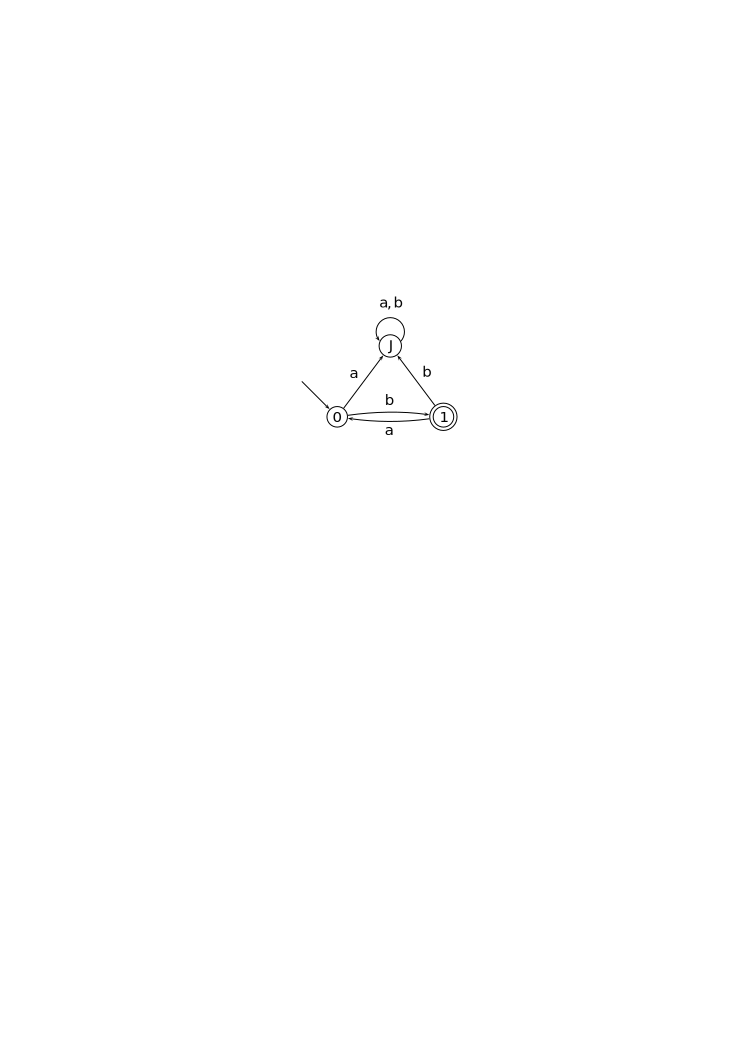
\includegraphics[width=0.7\linewidth]{automaten/Loesung2.pdf}
	\end{figure}
\end{frame}

% TODO: Fix dirty hack in thwregex.sty, where I changed line 42 to print star in math-mode
% 		because otherwise the star was always raised in my config.
%	COmment(Daniel): Reverted your change. No problems whatsoever.
%		Use \rx everywhere

% Fuck you, Latex. In my algo tutorial slides, this isn't necessary. Why here then!?
\begin{frame}[t]
	\fakeframetitle{\only<2->{Grenzen endlicher Akzeptoren}}
	Gibt es einen endlichen Akzeptor $A$ mit $$L(A) = \set{ \word a^k\word b^k \Mid k\in \N_0 }?$$
	\pause
	Nein! Warum nicht? \visible<3->{Endliche Automaten können nicht unendlich weit „zählen“!}\\
	
	Gibt es einen endlichen Akzeptor, der alle gültigen Klammerausdrücke erkennt?\\ \pause
	Nein, aus dem selben Grund.
	\begin{figure}[H]
		\includegraphics[scale=0.5]{xkcd/tags_1144}
		\caption{ \texttt{\url{https://www.xkcd.com/1144/}} }
	\end{figure}
	\pause
	Kontextfreie Grammatiken \enquote{können also mehr} als endliche Akzeptoren.\\
	Wir wollen nun ein \enquote{gleichmächtiges} Konzept zu Akzeptoren.
\end{frame}

\section{Reguläre Ausdrücke}
\subsection{Definition}

\begin{frame}{Disclaimer!}
	\begin{center}
		\Large
			\bfalert{\Huge ACHTUNG!} \\ \medskip
		
		Gemeint sind \textbf{NICHT} sog. \emph{Regular Expressions}, die ihr vllt. aus Programmiersprachen kennt! \\ \bigskip
		
		{\normalsize (Die sind ähnlich, aber eben nicht das gleiche.)}
	\end{center}
\end{frame}

\begin{frame}{Reguläre Ausdrücke}
	Wir können uns reguläre Ausdrücke zusammenbauen aus
	\begin{itemize}
		\item den einzelnen Symbolen $x$ aus $A$ \pause
		\item zwei regulären Ausdrücken $R_1$ und $R_2$ mit $$\rx(R_1 R_2\rx) \qquad \text{ oder } \qquad \rx(R_1\rx|R_2\rx)$$ \pause
		\item einem Stern $R\rx*$ \pause
		\item oder dem leeren Ausdruck $\rx O$ \pause
	\end{itemize} 
	Klammern dürfen nach den Klammerregeln weggelassen werden:\\
	Stern vor „Punkt“ {\small (in diesem Fall unsichtbar)} vor Strich.
\end{frame}

\begin{frame}{Reguläre Ausdrücke}
	\begin{Beispiel}
		Sei $ A = \{ \word a, \word b, \word c\}$. Dann sind gültige reguläre Ausdrücke über $A$:\\
		$\rx{abc}$\\
		$\rx{a|b|c}$\\
		$\rx{(ab)*}$\\
		$\rx{O*}$
	\end{Beispiel}
\end{frame}


\begin{frame}{Sprache eines Ausdruckes}
	Die durch $R$ beschriebene Sprache $\lang{R}$ ist wie folgt definiert:
	\begin{itemize}
		\item $\lang{\rx{O}} = \emptyset$
		\item $\lang{x}=\{x\} \quad (\text{für }x\in A)$
		\item $\lang{R_1 \rx| R_2} = \lang{R_1} \cup \lang{R_2}$
		\item $\lang{R_1 R_2} = \lang{R_1} \cdot \lang{R_2}$
		\item $\lang{R\rx*} = \lang{R}^*$
	\end{itemize} 

	\bigskip
	Eine Sprache, für die es einen beschreibenden regulären Ausdruck gibt, nennt man \textbf{regulär}.
\end{frame}

\begin{frame}{Sprache eines Ausdruckes}
	\begin{Beispiel}
		\begin{itemize}
			\item $\lang{\rx{a}} = \{\word a\}$. \pause
			\item $\lang{\rx{ab}} = \lang{\rx{a}} \cdot \lang{\rx{b}} = \{\word a\word b\}$. \pause
			\item $\lang{\rx{a|b}} = \lang{\rx{a}}\cup\lang{\rx{b}} = \{\word a,\word b\}$. \pause
			\item $\lang{\rx{(a|b)*}} = \lang{\rx{a|b}}^* = \{\word a,\word b\}^*$. \pause
			\item $\lang{\rx{(a*b*)*}} = \lang{\rx{a*b*}}^* = \left(\lang{\rx{a*}}\lang{\rx{b*}}\right)^* 
			= \left(\lang{\word a}^*\lang{\word b}^*\right)^* = \left(\{\word a\}^* \· \{\word b\}^*\right)^*$\\
			$= \{\word a,\word b\}^*$.  
		\end{itemize}
	\end{Beispiel}
	\pause
	\begin{block}{Aufgabe}
		Gebt einen regulären Ausdruck $R$ an mit $\lang{R} = $  
		\begin{itemize}
			\item die Sprache aller binären Zweierpotenzen \\ \visible<+->{}
				  \visible<+-|handout:2>{\impl $R = \rx{0*10*}$}
			\item die Sprache aller geraden Binärzahlen \\
				  \visible<+-|handout:2>{\impl $R = \rx{(0|1)*0}$}
		\end{itemize}
	\end{block}
\end{frame}

\begin{frame}{Aufgabe: Reguläre Ausdrücke}
	In dieser Aufgabe geht es um die formalen Sprachen
	$$L_1 = \set{\word a^k \word b^m \Mid k, m \in \N_0 }, \qquad L_2 = \set{\word b^k \word a^m \Mid k, m \in \N_0 }.$$
	Gebt für jede der folgenden formalen Sprachen $L$ je einen regulären Ausdruck $R$ an mit $ \langle R \rangle = L$.
	\begin{itemize}
		\item $L = L_1 \cup L_2$ \\
			\visible<2-|handout:2>{$ \rx{a*b*|b*a*}$}
		\item $L = L_1 \cap L_2$ \\
			\visible<3-|handout:2>{$ \rx{a*|b*}$}
		\item $L = L_1\cdot L_2$ \\
			\visible<4-|handout:2>{$ \rx{a*b*b*a*}$ oder $\rx{a*b*a*}$}
		\item $L = L_1^*$ \\
			\visible<5-|handout:2>{$ \rx{(a*b*)*}$ oder $\rx{(a|b)*}$}
	\end{itemize}
\end{frame}

\begin{frame}{Aufgabe: Sprachen regulärer Ausdrücke}
	\begin{itemize}
		\item $\lang{\rx{(a|b)*abb(a|b)*}} = \visible<2-|handout:2>{\{\word a, \word b\}^* \cdot \{\word a\word b\word b\} \cdot \{\word a, \word b\}^*}$
		\item $\lang{\rx{a**}} = \visible<3-|handout:2>{\{\word a\}^*}$
		\item $\lang{\visible<4-|handout:2>{R\rx{(}R\rx{)*}}} = \lang{R}^+$ \quad (für bel. reg. Ausdruck $R$)
		\item $\lang{\visible<5-|handout:2>{\rx{O*}}} = \{\eps\}$
		\item $\lang{\visible<6-|handout:2>{\rx{a*ba*ba*b(a|b)*}}} = \set{ w \in \{\word a, \word b\}^* \Mid \size{w}_{\word b} > 2 } $
		\item $\lang{\visible<7-|handout:2>{\rx{b*a*}}} =$ Sprache aller Wörter über $\set{\word a, \word b}$, in denen das Teilwort \word{ab} nicht vorkommt.
	\end{itemize}
\end{frame}


% Dieses Jahr nicht
%input{../Bloecke/StrukturelleInduktion}

\begin{frame}	
	\begin{block}{Was ihr nun wissen solltet}
		\begin{itemize}
			\item Reguläre Ausdrücke
			\item Rechtslineare Grammatiken
		\end{itemize}
	\end{block}
	
	\begin{block}{Was nächstes Mal kommt}
		\begin{itemize}
			\item Turingmaschinen - Mächtiger wird es nicht mehr!
		\end{itemize}
	\end{block}
\end{frame}

\lastframe{0.6}{30}{xkcd/automation_1319.png}{http://www.xkcd.com/1319}
\xkcdframe{0.5}{30}{xkcd/houston_1438.png}{http://www.xkcd.com/1438}{Oh, hi mom. No, nothing important, just work.}

\slideThanks

\end{document}